\scanpage{104}
\mspage{103}%
tions on $F$ (decreasing, \inserted{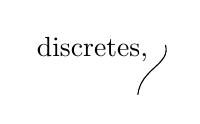
\begin{tikzpicture}[baseline=-.2ex,x=1em,y=1em]
\node[anchor=base west] at (0,.55) {discrete\handwritten{s,}};
\draw (5,.95) .. controls (5.2,.25) and (4.1,.1) .. (4,-.85);
\end{tikzpicture}} indexed by $\underline{Z}$) compatible with tensor products (using the ev\deleted{\unsure{o|q}}\handwritten{i}dent notion of the tensor\deleted{s} produ\rlap{q}ct of two fi\rlap{g}l\rlap{l}tered vector spaces). One will note that\deleted{e} such a datum will no longer be expressible by a homomorphism from a certain algebraic group into $G$ (the Galois group of $\underline{C}$ at $F$), for the category of finite-dimensional vect\rlap{r}o\rlap{o}r spaces over $k$, equipped with a\rlap{\tikz[baseline=0pt,x=1em,y=1em]{\draw (.05,.8)--(.08,.96);}} discrete decreasing filtration indexed by $\underline{Z}$, is not an abelian category\rlap{\tikz[baseline=0pt,x=1em,y=1em]{\draw (0,-.55)--(.05,-.7);\fill (-.04,-.85) circle (.045);}} (bimorphisms are not isomorphisms\handwritten{!}). But to such a datum is associated a se\deleted{e}cond fibre functor\margin{\handwritten{$F'$}} $\inserted{\unsure{F|\mathbb{F}}'(V)=}\rlap{\handwritten{\tikz[baseline=0pt,x=1em,y=1em]{\draw (.35,.4) .. controls (.7,-.25) and (-3.5,-.2) .. (-3.6,-.6) .. controls (-3.8,-.8) and (-3.75,-1.1) .. (-3.6,-1.15);}}}\operatorname{Gr}F(V)$, taking values this time in graded vector spaces (NB $F$ plays the role of \deleted{Hodge, $F'$} De Rham cohomology, $F'$ th\rlap{l}a\rlap{e}t of Hodge cohomology\deleted{\unsure{)}}, equipped with the \deleted{total} grading \inserted{\handwritten{by $p$}}). The datum of $F'$ then corresponds to a \inserted{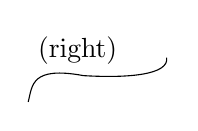
\begin{tikzpicture}[baseline=-.2ex,x=1em,y=1em]
\node[anchor=base west] at (0,.5) {\handwritten{(right)}};
\draw (5,.5) .. controls (5.1,-.1) and (3.7,-.25) .. (2,-.15) .. controls (.1,.2) and (.15,-.5) .. (0,-1.1);
\end{tikzpicture}} torsor $P$ under $G$, the corresponding Galois group $G'$ being obtained from $G$ by twisting by $P$. The grading of $F'$ corresponds to a homomorphism $i_{\handwritten{1}}:\underline{G}_m\handwritten{\longrightarrow}G'$. Let us then consider on $F'$ the decreasing filtration associated with its gra\unsure{\rlap{u}d|d}\rlap{d}ing, and let $H'_{i_{\handwritten{1}}}=\underline{\operatorname{Aut}}\,\underline{\mathrm{filt}}^{\handwritten{!}}(F')\handwritten{\subset}\underline{\operatorname{Aut}}(F')=G'$ be the subgroup scheme of $G$ which corresponds to the \inserted{$\otimes$-}\rlap{\handwritten{\tikz[baseline=0pt,x=1em,y=1em]{\draw (-.9,.2) .. controls (-.4,.05) and (-.1,-.7) .. (-.2,-.8) .. controls (-.5,-.7) and (.1,-.2) .. (.7,.3);}}}automorphisms of $F'$ (or rather of the $F'_{k'}$, $k'$ an arbitrary $k$-algebra) which respect its filtration\inserted{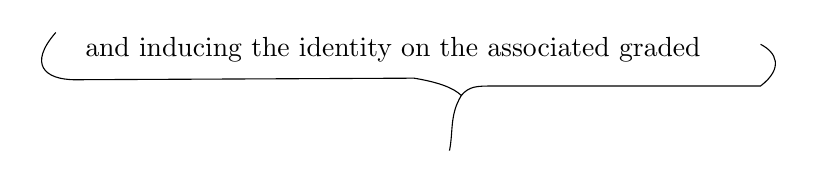
\begin{tikzpicture}[baseline=-.2ex,x=1cm,y=1cm]
\node[anchor=base west] at (0,.3) {\handwritten{and inducing the identity on the associated graded}};
\draw (-.25,.6) .. controls (-.6,.2) and (-.4,0) .. (0,0) -- (4.3,.02) .. controls (4.6,-.03) and (4.8,-.1) .. (4.9,-.2) .. controls (5,-.08) and (5.1,-.08) .. (5.3,-.08) -- (8.7,-.08) .. controls (9,.15) and (8.9,.35) .. (8.7,.45);
\draw (4.9,-.2) .. controls (4.75,-.45) and (4.8,-.65) .. (4.75,-.9);
\end{tikzpicture}}; it is canonically determined by $i_{\handwritten{1}}$. One can also look at the subscheme
\[
Q=\underline{\operatorname{Isom}}\,\underline{\mathrm{filt}}^{\handwritten{!}}(F,F')\handwritten{\subset}P=\underline{\operatorname{Isom}}(F,F')
\]
of the scheme $P$ of $\otimes$-isomorphisms of $F$ with $F'$, \deleted{formed of} which corresponds to the \rlap{i}a\rlap{s}u\rlap{t}omorphisms respecting the filtrations of $F$ and $F'$\inserted{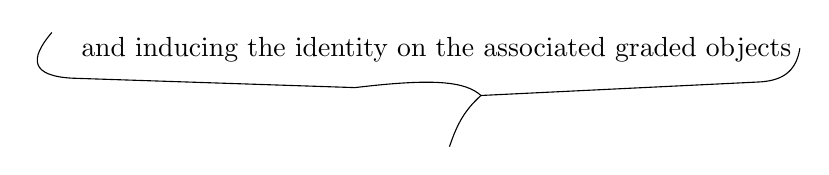
\begin{tikzpicture}[baseline=-.2ex,x=1cm,y=1cm]
\node[anchor=base west] at (0,.3) {\handwritten{and inducing the identity on the associated graded objects}};
\draw (-.25,.6) .. controls (-.55,.25) and (-.5,.05) .. (0,.02) -- (3.6,-.1) .. controls (4.6,.02) and (5,-.02) .. (5.2,-.2) -- (8.7,-.03) .. controls (9,-.02) and (9.2,.08) .. (9.25,.4);
\draw (5.2,-.2) .. controls (5,-.38) and (4.9,-.55) .. (4.8,-.85);
\end{tikzpicture}}. This is a priori a \deleted{right}\inserted{\handwritten{left}} pseudo-torsor under $H'$, \rlap{\tikz[baseline=0pt,x=1em,y=1em]{\draw (.15,.25) .. controls (.2,0) and (.1,-.2) .. (.17,-.5);}}i.e. it is empty or a right torsor under $H'$. \uuline{One would need to prove} that it is indeed a torsor (i.e. that over a suitable extension $k'$ of $k$, one can \rlap{y}find an isomorphism\margin{\handwritten{\tikz[baseline=0pt,x=1em,y=1em]{\draw (0,0)--(.15,.18);}}} of $F_{k'}$ with $F'_{k'}$ \uline{respecting the filtrations}). Thus one finds a restriction o\rlap{e}f the group of operators (on the \deleted{right}\inserted{\handwritten{left}}) $G'$ of $P$ to the subgroup $H'$,
